\chapter{Hidden Markov Models}
Many of the techniques we've considered so far in this book have been motivated by the \textit{types} of data we could expect to work with. For example, the supervised learning techniques (forms of regression, neural networks, support vector machines, etc.) were motivated by the fact that we had labelled training data. We ventured into clustering to group unlabelled data and discussed dimensionality reduction to handle overly high-dimensional data. In the previous chapter, we examined techniques for managing \textit{incomplete} data with latent variable models. In this chapter we turn to a technique for handling
temporal data.

\section{Motivation}

One major type of data we have not yet paid explicit attention to is \textit{time series} data. Most of the information we record comes with some sort of a timestamp. For example, any time we take an action online, there is a high probability that the database storing the data also tracks it with a timestamp. Physical sensors in the real world always record timestamps because it would be very difficult to make sense of their information if it is not indexed by time. When we undergo medical exams, the results are recorded along with a timestamp. It's almost inconceivable at this point that we would record information without also keeping track of when that data was generated, or at the very least when we saved that data.

For these reasons, its interesting to develop models that are specialized to temporal data.
% As we've already discussed, it's a near-universal feature because we so frequently record timestamp information. It's difficult to imagine a data set that couldn't come with timestamps attached to the individual data points.
%
Certainly, 
time encodes a lot of information that we take for granted about the physical and digital worlds. For example, if the sensors on a plane record the position of the plane at a specific point in time, we would expect the surrounding data points to be relatively similar, or at least move in a consistent direction. In a more general sense, we expect that time constrains other attributes of the data in specific ways.

% Because we know time posseses these unique properties, it follows that we should exploit them to create more expressive models.

In this chapter, we will focus on one such model known as a \textbf{Hidden Markov Model} or \textbf{HMM}. At a high level, the goal of an HMM is to model the state of an entity over time, with the caveat that we never actually observe the state itself. Instead, we observe a data point $\textbf{x}_t$ at each time step (often called an `emission' or `observation') that depends on
the state $\textbf{s}_t$. For example, we could model the position of a robot over time given a noisy estimation of the robot's current position at each time step. Furthermore, we will assume that one state $\textbf{s}_t$ transitions to the next state $\textbf{s}_{t+1}$ according to a probabilistic model. Graphically, an HMM looks like Figure \ref{fig:HMM-DGM}, which encodes the relationships between emissions and hidden states.  Here, there are $n$ time steps in total.
%
\begin{figure}
    \centering
    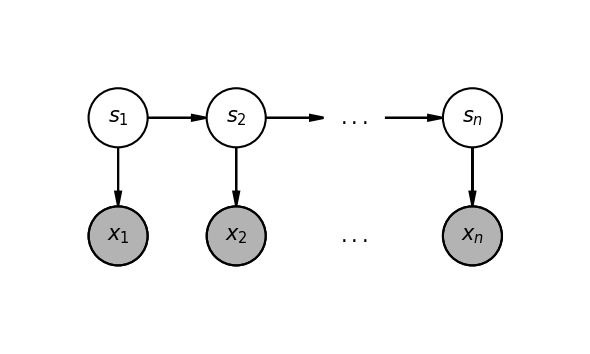
\includegraphics[width=0.5\paperwidth]{../HiddenMarkovModels/fig/HMM_DGM.png}
    \caption{The directed graphical model for an HMM.}
    \label{fig:HMM-DGM}
\end{figure}

We will probe HMMs in more detail over the course of the chapter, but for now let's consider their high-level properties.

\begin{mlcube}{Hidden Markov Models}
First, HMMs handle discrete states, and for the purpose of this text, we will only consider discrete-valued emissions as well. Second, since a HMM does not have access to the states, these are hidden (or latent) and in this sense we can view training as ``unsupervised.'' Finally, we assume a probabilistic relationship between hidden states and observed emissions as well as the transitions between hidden states.
\begin{center}
    \begin{tabular}{c|c|c}
    \textit{\textbf{Domain}} & \textit{\textbf{Training}} & \textit{\textbf{Probabilistic}} \\
    \hline
    Discrete & Unsupervised & Yes \\
    \end{tabular}
\end{center}
\end{mlcube}
\readernote{Models that treat continuous state variables are commonly referred to as dynamical systems.}

\section{Applications}

Unsurprisingly, there are many applications for models like HMMs that explicitly account for time and unobserved states, especially those that relate to the physical world. Examples include:
\begin{enumerate}
    \item The position of a robot arm when its movements may be non-deterministic and sensor readings are noisy. [State = robot arm position; observation  = sensor reading]
    \item Speech recognition. [State = phoneme; observation = sound]
    \item Analyzing sequences that occur in the natural world, such as DNA [State = codon, a genetic code in a DNA molecule; observation= one of the four bases, i.e., A, C, T, or G]
\end{enumerate}

\section{HMM Data, Model, and Parameterization}

As explained above, HMMs model the state of an entity over time given some noisy observations, as shown in Figure \ref{fig:HMM-DGM}.

\subsection{HMM Data}

The data for a HMM consists of the sequence of one-hot encoded emissions $\textbf{x}_1, ..., \textbf{x}_n$, for $n$ total time steps. Their corresponding states, $\textbf{s}_1, ..., \textbf{s}_n$, are latent and unobserved.

Each state corresponds to one of $K$ possible options, i.e., with one-hot coding,
$\textbf{s}_t \in \{0,1\}^K$. Each emission corresponds to one of $M$ possible options, with one-hot coding, $\textbf{x}_t \in \{0,1\}^M$.
% It's our goal to infer the hidden states.

\readernote{In general the observed emissions don't have to be discrete, but for the sake of being explicit, we present the discrete interpretation here.}

% Note that a single \textit{data point} consists of a sequence of $n$ emissions $\textbf{x}_1, ..., \textbf{x}_n$.

A data set has $N$ data points, meaning $N$ sequences where each sequence is composed of $n$ emissions (in general they can be of different lengths, we assume same length for simplicity).
To summarize:
%
\begin{itemize}
	\item A data set consists of $N$ sequences.
	\item Each sequence is composed of $n$ observed emissions $\textbf{x}_1, ..., \textbf{x}_n$.
%	\item It's our goal to infer the hidden states $\textbf{s}_1, ..., \textbf{s}_n$ for each sequence.
	\item Each emission $\textbf{x}_{t}$ takes on one of $M$ possible values.
	\item Each hidden state $\textbf{s}_{t}$ take on one of $K$ possible values.
\end{itemize}

\subsection{HMM Model Assumptions}


In modeling the joint distribution over hidden states and observed emissions
\begin{equation} \label{large-joint}
	p(\textbf{s}_1, ..., \textbf{s}_n, \textbf{x}_1, ..., \textbf{x}_n) = p(\textbf{s}_1, ..., \textbf{s}_n) p(\textbf{x}_1, ..., \textbf{x}_n | \textbf{s}_1, ..., \textbf{s}_n),
\end{equation}
%
the HMM model makes the following two assumptions:
%
\begin{itemize}
    \item[1.] State $\textbf{s}_{t+1}$ depends only on the previous state $\textbf{s}_t$:
	    \begin{align*}
	    	p(\textbf{s}_{t+1} | \textbf{s}_{1}, ..., \textbf{s}_{t}, \textbf{x}_{1}, ..., \textbf{x}_{t}) = p(\textbf{s}_{t+1} | \textbf{s}_{t}) 
	    \end{align*}
            This is the \textit{Markov Property}, and it means that given knowledge of the state at the previous time step, we can ignore all other earlier states and emissions. Here, we also assume the transition is \textit{stationary}, so that the transition model doesn't depend on time.
            %l
          \item[2.] At each time step $t$, the observed emission $\textbf{x}_t$ depends only on the current state $\textbf{s}_t$:
            %
    	\begin{align*}
	    	p(\textbf{x}_{t} | \textbf{s}_{1}, ..., \textbf{s}_{t}, \textbf{x}_{1}, ..., \textbf{x}_{t-1}) = p(\textbf{x}_{t} | \textbf{s}_{t}) 
	    \end{align*}
          \end{itemize}
          
          \readernote{The Markovian assumption for transitions, as well as the fact that we don't observe the true states, gives rise to the \textit{Hidden Markov Model} name.}

          These two assumptions allow us to factorize the large joint distribution given by Equation \ref{large-joint} as follows:
          %
\begin{equation} \label{factorized-joint}
	p(\textbf{s}_1, ..., \textbf{s}_n) p(\textbf{x}_1, ..., \textbf{x}_n | \textbf{s}_1, ..., \textbf{s}_n) = p(\textbf{s}_1) \prod_{t=1}^{n-1} p(\textbf{s}_{t+1} | \textbf{s}_t) \prod_{t=1}^{n} p(\textbf{x}_t | \textbf{s}_t)
      \end{equation}
      
This factorization will prove important for making HMM training and inference tractable.

\subsection{HMM Parameterization} \label{hmm-parameterization}

Now that we understand the form of the data as well as the modeling assumptions made by a HMM, we can specify the model parameterization explicitly. Referencing the factorized joint distribution from Equation \ref{factorized-joint}, we will need three distinct sets of parameters.
%
\begin{itemize}
	\item[1.]  Parameters for the prior over the initial hidden state $p(\textbf{s}_1)$. This will be denoted $\boldsymbol{\theta} \in [0,1]^{K}$, with $\sum_k\theta_k=1$, such that:
	\begin{align*}
		p(\textbf{s}_1 = k) = \theta_k.
	\end{align*}
%
	\item[2.] Parameters for the transition probabilities between states $p(\textbf{s}_{t+1} | \textbf{s}_t)$. This will be denoted $\textbf{T} \in [0,1]^{K \times K}$, with $\sum_j T_{i,j}=1$ for each $i$, such that:
	\begin{align*}
		p(\textbf{s}_{t+1} = j | \textbf{s}_t = i) = T_{i,j},
	\end{align*}
	where $T_{i,j}$ is the probability of transitioning from state $i$ to state $j$.
%
	\item[3.] Parameters for the conditional probability of the emission, $p(\textbf{x}_t | \textbf{s}_t)$,  given the state. This will be denoted $\boldsymbol{\pi} \in [0,1]^{K \times M}$, with $\sum_m \pi_{k,m}=1$ for each $k$, such that:
	\begin{align*}
		p(\textbf{x}_t = m | \textbf{s} = k) = \pi_{k, m}.
	\end{align*}

	For each state, there is a distribution on possible emissions.
        %has an $M$-dimensional vector describing the probability of an emission given that state.
\end{itemize}

In sum, we have three sets of parameters $\boldsymbol{\theta} \in [0,1]^{K}$, $\textbf{T} \in [0,1]^{K \times K}$, and $\boldsymbol{\pi} \in [0,1]^{K \times M}$ that we need to learn from our data set.
Then, using a trained model, we will be able to perform several types of inference over our hidden states, as detailed next.

\section{Inference in HMMs}


We will see how to estimate the parameters of a HMM (``training'') in Section~\ref{sec:hmmEM}. For now we want to understand how to do efficient inference in HMMs. Given parameters $\boldsymbol{\theta}, \textbf{T}$, and $\boldsymbol{\pi}$, and given a sequence of observations, $\textbf{x}_1, ..., \textbf{x}_n$ (or $\textbf{x}_1, ..., \textbf{x}_t$) there are various queries we may like to perform:
%
\begin{itemize}
	\item ``p(seq)'' $p(\mathbf{x}_1,\ldots,\mathbf{x}_n)$  (what is the distribution on sequences of emissions?)
	\item Prediction $p(\mathbf{x}_{t+1}|\mathbf{x}_1,\ldots,\mathbf{x}_t)$ (what is the prediction of the next emission given what is known so far?)
	\item Smoothing $p(\mathbf{s}_t|\mathbf{x}_1,\ldots,\mathbf{x}_n), t\leq n$ (after the fact, what do we predict for some earlier state?)
	\item Transition $p(\mathbf{s}_t,\mathbf{s}_{t+1}|\mathbf{x}_1,\ldots,\mathbf{x}_n), t+1\leq n$ (after the fact, what do we predict for the joint distribution on some pair of temporally adjacent states?)
        \item Filtering $p(\mathbf{s}_t|\mathbf{x}_1,\ldots,\mathbf{x}_t)$ (what is the prediction, in real-time, of the current state?)
          %
          \item Best path $\max p(\mathbf{s}_1,\ldots,\mathbf{s}_n|\mathbf{x}_1,\ldots,\mathbf{x}_n)$ (after the fact, what is the most likely sequence of states?)
\end{itemize}

For just one example, let's consider smoothing $p(\textbf{s}_t | \textbf{x}_1, ..., \textbf{x}_n)$. To
compute this 
would require marginalizing over all the unobserved states other than $\textbf{s}_{t}$, as follows:
\begin{align*}
  p(\textbf{s}_t |\textbf{x}_1, ..., \textbf{x}_n) &\propto p(\textbf{s}_t, \textbf{x}_1, ..., \textbf{x}_n)\\
                                                   &=\sum_{s_1,\ldots,s_{t-1},s_{t+1},\ldots,s_n} p(\textbf{s}_1, \ldots, \textbf{s}_n, \textbf{x}_1, \ldots, \textbf{x}_n)
  \\
                                                   &=\sum_{s_1,\ldots,s_{t-1},s_{t+1},\ldots,s_n}p(\textbf{s}_1) \prod_{t=1}^{n-1} p(\textbf{s}_{t+1} | \textbf{s}_t) \prod_{t=1}^{n} p(\textbf{x}_t | \textbf{s}_t).
\end{align*}

Without making use of variable elimination, this requires summing over all possible states other than $t$, which is very costly.
%
Moreover, suppose we then query this for another state. We'd need to sum again over all the states except for this new state,
which duplicates a lot of work.
%
Rather than performing these summations over and over again, we can instead ``memoize'' (or reuse) these kinds of summations using the Forward-Backward algorithm. This  algorithm also makes uses of variable elimination to improve the efficiency of inference.

\subsection{ The Forward-Backward Algorithm}


The Forward-Backward algorithm uses variable elimination methods to compute two sets of quantities, that we refer to as the ``alpha'' and ``beta'' values. The algorithm makes elegant use of dynamic programming (breaking down optimization problem into sub-problems, solving each sub-problem a single time, and storing the solutions). It can be viewed as a preliminary inference step such that the alpha and beta values can then be used for all inference tasks of interest as well as within EM for training a HMM model.

The Forward-Backward algorithm is also an example of a \textit{message-passing} scheme, which means we can conceptualize it as passing around compact messages along edges of the graphical model that corresponds to a HMM.
%The goal is to avoid duplicating work, instead using the messages directly. If you've encounted dynamic programming before, the Forward-Backward Algorithm is an example.
%
The algorithm passes messages forwards and backwards through `time', meaning up and down the chain shown in the graphical model representation in Figure~\ref{fig:HMM-DGM}. The forward messages are defined at each state as $\alpha_t(\textbf{s}_t)$, while the backward messages are defined at each state as $\beta_t(\textbf{s}_t)$. The overarching idea is to factor the joint distribution $$p(\textbf{x}_1,\dots,\textbf{x}_n,\textbf{s}_t) = p(\textbf{x}_1,\dots,\textbf{x}_t,\textbf{s}_t) p(\textbf{x}_{t+1},\dots,\textbf{x}_n|s_t)$$ because the factored terms can be efficiently computed. Let's define these $\alpha$ and $\beta$ terms explicitly.

The $\alpha_t$'s represent the joint probability of all our observed emissions from time $1,...,t$ as well as the state at time $t$:
%
\begin{equation} \label{unfactorized-alphas}
	\alpha_t(\textbf{s}_t) = p(\textbf{x}_1, ..., \textbf{x}_t, \textbf{s}_t)
\end{equation}
Graphically, the $\alpha_t$'s are capturing the portion of the HMM  shown in Figure \ref{fig:HMM-DGM-alpha}.


\begin{figure}[h!]
    \centering
    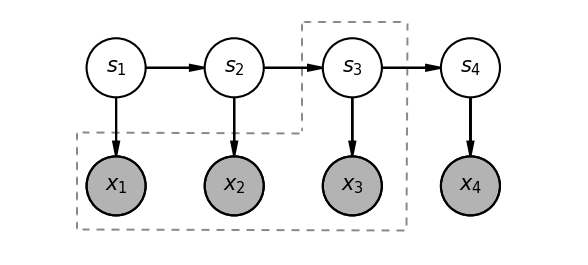
\includegraphics[width=0.5\paperwidth]{../HiddenMarkovModels/fig/HMM_DGM_alpha.png}
    \caption{$\alpha_t$'s capture the joint probability for the boxed portion; shown for $\alpha_3(\mathbf{s}_3)$}
    \label{fig:HMM-DGM-alpha}
\end{figure}



% Note that Equation \ref{unfactorized-alphas} is an unfactorized joint probability over observed emissions and a hidden state.

We can factorize this joint probability using what we know about the conditional independence properties of HMMs as follows:
%
\begin{align} 
  \alpha_t(\textbf{s}_t) &= p(\textbf{x}_1, ..., \textbf{x}_t, \textbf{s}_t) \notag \\
                         &=p(\textbf{x}_t|\textbf{x}_1,\ldots,\textbf{x}_{t-1},\textbf{s}_t)p(\textbf{x}_1,\ldots,\textbf{x}_{t-1},\textbf{s}_t)\notag \\
                         &=p(\textbf{x}_t|\textbf{s}_t)\sum_{s_{t-1}}p(\textbf{x}_1,\ldots,\textbf{x}_{t-1},\textbf{s}_{t-1},\textbf{s}_t) \label{eq:hmmdcp1} \\
                         &=p(\textbf{x}_t|\textbf{s}_t)\sum_{s_{t-1}}p(\textbf{s}_t|\textbf{x}_1,\ldots,\textbf{x}_{t-1},\textbf{s}_{t-1})p(\textbf{x}_1,\ldots,\textbf{x}_{t-1},\textbf{s}_{t-1})\\
  &= p(\textbf{x}_t | \textbf{s}_t) \sum_{s_{t-1}} p(\textbf{s}_t | \textbf{s}_{t-1}) \alpha_{t-1}(\textbf{s}_{t-1})\label{eq:alpharecurse}
\end{align}

The first term in Equation~\eqref{eq:hmmdcp1} follows from the Markov property, and for the second term we've expressed this joint probability by explicitly introducing $\textbf{s}_{t-1}$ and marginalizing out over this variable. Equation~\ref{eq:alpharecurse} follows from the Markov property, and by
substituting for the definition of the alpha value. 



Notice that our expression for $\alpha_t(\textbf{s}_t)$ includes the expression for $\alpha_{t-1}(\textbf{s}_{t-1})$, which is the $\alpha$ from the previous time step.
This means we can define our messages \textit{recursively}.
%
After we've computed the $\alpha$'s at one time step,
we \textit{pass} them forwards along the chain and use them in the computation of
alpha values for the next time step.
%
In other words, we compute the $\alpha$ values for period 1, then pass that message along to compute the $\alpha$ values  in period 2, and so forth until we reach the end of the chain and have all the $\alpha$'s in hand.

\readernote{These $\alpha$ values are used both for inference and training a HMM via EM (in the E-step)}

At this point, we've handled the forward messages, which send information from the beginning to the end of the chain. In the backward portion, we also send information from the end of the chain back to the beginning. In this backward message pass, we will compute our $\beta$ values.
%
The $\beta_t$'s represent the joint probability over all the observed emissions from time $t+1, ..., n$ conditioned on the state at time $t$:
\begin{equation} \label{unfactorized-betas}
	\beta_t(\textbf{s}_t) = p(\textbf{x}_{t+1}, ..., \textbf{x}_n | \textbf{s}_t)
\end{equation}
Graphically, this means that the $\beta_t$'s are capturing the portion of the HMM shown in Figure \ref{fig:HMM-DGM-beta}.
%
\begin{figure}[b!]
    \centering
    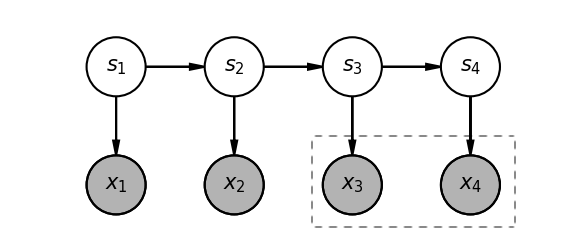
\includegraphics[width=0.5\paperwidth]{../HiddenMarkovModels/fig/HMM_DGM_beta.png}
    \caption{$\beta_t$'s capture the joint probability for the boxed portion of the HMM. Shown here for $\beta_2(\mathbf{s}_2)$} 
    \label{fig:HMM-DGM-beta}
\end{figure}



We can factorize Equation~\ref{unfactorized-betas} in a similar way to how we factorized the distribution described by the $\alpha$'s:
%
\begin{align}
  \beta_t(\textbf{s}_t) &= p(\textbf{x}_{t+1}, ..., \textbf{x}_n | \textbf{s}_t) \notag \\
&=\sum_{\textbf{s}_{t+1}} p(\textbf{x}_{t+1}, ..., \textbf{x}_n, \textbf{s}_{t+1} | \textbf{s}_t) 
 \label{eq:dcp1hmm} \\
                        &= \sum_{\textbf{s}_{t+1}} p(\textbf{s}_{t+1} | \textbf{s}_t) p(\textbf{x}_{t+1} | \textbf{s}_t, \textbf{s}_{t+1}) p(\textbf{x}_{t+2}, ..., \textbf{x}_n | \textbf{x}_{t+1}, \textbf{s}_t,\textbf{s}_{t+1}) \label{eq:dcp2hmm} \\
&  = \sum_{\textbf{s}_{t+1}} p(\textbf{s}_{t+1} | \textbf{s}_t) p(\textbf{x}_{t+1} | \textbf{s}_{t+1})
p(\textbf{x}_{t+2}, ..., \textbf{x}_n | \textbf{s}_{t+1})
  \label{eq:dcp3hmm}\\
	&= \sum_{\textbf{s}_{t+1}} p(\textbf{s}_{t+1} | \textbf{s}_t) p(\textbf{x}_{t+1} | \textbf{s}_{t+1}) \beta_{t+1}(\textbf{s}_{t+1}). \label{eq:dcp4hmm}
\end{align}

Here, Equation~\eqref{eq:dcp1hmm} introduces $\textbf{s}_{t+1}$ and marginalizes out over this variable.
Equation~\eqref{eq:dcp2hmm} is the product rule (recall that $n\geq t+1$, so the third conditional probability starts at $x_{t+2}$). Equation~\eqref{eq:dcp3hmm} makes use of the Markov property in the last two terms. Equation~\eqref{eq:dcp4hmm} substitutes in the expression for $\beta_{t+1}$ from Equation~\eqref{unfactorized-betas}.

As we saw with our calculation of the $\alpha$'s, we can calculate $\beta$ recursively. This recursive definition enables us to propagate messages backward and compute the beta values
efficiently in one pass. In this case, we start at the end of the chain ($t=n$), and compute our $\beta$'s for each state by passing messages back toward the front.

To summarize, the Forward-Backward algorithm calculates the $\alpha$ and $\beta$ values as follows:\
%
\begin{align*}
	\alpha_t(\textbf{s}_t) &=
	\begin{cases} 
      p(\textbf{x}_t | \textbf{s}_t) \sum_{\textbf{s}_{t-1}} p(\textbf{s}_t | \textbf{s}_{t-1}) \alpha_{t-1}(\textbf{s}_{t-1}) & 1 < t \leq n \\
      p(\textbf{x}_1 | \textbf{s}_{1}) p(\textbf{s}_1) & \text{otherwise} \\
   \end{cases} \\
   \beta_t(\textbf{s}_t) &=
   \begin{cases} 
      \sum_{\textbf{s}_{t+1}} p(\textbf{s}_{t+1} | \textbf{s}_t) p(\textbf{x}_{t+1} | \textbf{s}_{t+1}) \beta_{t+1}(\textbf{s}_{t+1}) & 1 \leq t < n \\
      1 & \text{otherwise} \\
   \end{cases}
\end{align*}

\readernote{Notice that the base case for the $\beta$'s is $n$. This is a quirk of our indexing, and it ensures we have a defined $\textbf{s}_{n}$ when we pass messages back to calculate $\textbf{s}_{n-1},\textbf{s}_{n-2},\dots$.}

\subsection{Using $\alpha$'s and $\beta$'s for Training and Inference}

Now that we know how to compute these $\alpha$ and $\beta$ values,
let's see how to use them for inference.
%
Consider the product of the $\alpha$ and $\beta$ value at a specific time $t$:
%
\begin{align*}
	\alpha_t(\textbf{s}_t) \beta_t(\textbf{s}_t) = p(\textbf{x}_1, ..., \textbf{x}_t, \textbf{s}_t) p(\textbf{x}_{t+1}, ..., \textbf{x}_n | \textbf{s}_t) = p(\textbf{x}_1, ..., \textbf{x}_n, \textbf{s}_t).
\end{align*}

This is the joint distribution over all emissions and the state at time $t$. Using this as a building block, this can support many kinds of inference.


\subsubsection{p(Seq)}

For example, we might like to evaluate the joint distribution over the emissions.
%
\begin{equation} \label{joint-fn}
  p(\textbf{x}_1, ..., \textbf{x}_n) = \sum_{\textbf{s}_t}p(\textbf{x}_1, ..., \textbf{x}_n, \textbf{s}_t)=
\sum_{\textbf{s}_t}
  \alpha_t(\textbf{s}_t) \beta_t(\textbf{s}_t)
\end{equation}
where we can sum over the possible state values. This calculation be defined for any state $\textbf{s}_t$.

\subsubsection{Prediction}

Another common task is to predict the value of the next emission given the previous emissions.
%
\begin{align*} 
&	p(\textbf{x}_{t+1} | \textbf{x}_1, ..., \textbf{x}_t)
\end{align*}

To compute this we can sum over state $\textbf{s}_t$ and the
next state $\textbf{s}_{t+1}$ as follows:
%
\begin{align}
  p(\textbf{x}_{t+1} | \textbf{x}_1, ..., \textbf{x}_t) &\propto   p(\textbf{x}_1, ..., \textbf{x}_t, \textbf{x}_{t+1} )\notag
  \\
                                                        &=  \sum_{\textbf{s}_t} \sum_{\textbf{s}_{t+1}} p(\textbf{x}_1, ..., \textbf{x}_t, \textbf{x}_{t+1}, \textbf{s}_t, \textbf{s}_{t+1})\label{eq:dp33hmm}
  \\
  &= \sum_{\textbf{s}_t} \sum_{\textbf{s}_{t+1}} p(\textbf{x}_1, ..., \textbf{x}_t, \textbf{s}_t) p(\textbf{s}_{t+1} | \textbf{x}_1, ..., \textbf{x}_t, \textbf{s}_t) p(\textbf{x}_{t+1} | \textbf{x}_1, ..., \textbf{x}_t, \textbf{s}_t,\textbf{s}_{t+1}) \label{eq:dp44hmm}\\
	&= \sum_{\textbf{s}_t} \sum_{\textbf{s}_{t+1}} \alpha_{t}(\textbf{s}_t) p(\textbf{s}_{t+1} | \textbf{s}_t) p(\textbf{x}_{t+1} | \textbf{s}_{t+1}).\label{eq:dp55hmm}
\end{align}

Here, Equation~\eqref{eq:dp33hmm} follows by introducing states $\textbf{s}_t$  and $\textbf{s}_{t+1}$ and marginalizing out over them. Equation~\eqref{eq:dp44hmm} follows from the product rule, and Equation~\eqref{eq:dp55hmm} by using the Markov property  in two places and substituting for $\alpha_{t}(\textbf{s}_t)$.

%Again, we recover a proportional result from this operation. We can use the softmax over the emissions states to normalize.


\subsubsection{Smoothing}

Smoothing is the problem of predicting the state at time $t$ given all the observed emissions.  We can think about this as updating the beliefs that we would have had in real-time, given emissions up to and including $t$, given {\em all} observed evidence up to period $n$. Hence the phrasing ``smoothing.''
%
For this, we have 
\begin{equation} \label{smoothing-fn}
	p(\textbf{s}_t | \textbf{x}_1, ..., \textbf{x}_n) \propto p(\textbf{x}_1, ..., \textbf{x}_n, \textbf{s}_t) = \alpha_t(\textbf{s}_t) \beta_t(\textbf{s}_t).
\end{equation}

%Notice that the proportionality of the smoothing operation means we can normalize to recover %probabilities by taking the softmax over the possible values for the state $\textbf{s}_t$. 


\subsubsection{Transition}

Finally, we may wish to understand the joint distribution
on states $\textbf{s}_t$ and $\textbf{s}_{t+1}$ given all the observed evidence.
%
\begin{align} 
  p(\textbf{s}_{t}, \textbf{s}_{t+1} | \textbf{x}_1, ..., \textbf{x}_n) &
                                                                    \propto      p(\textbf{s}_{t}, \textbf{s}_{t+1} , \textbf{x}_1, ..., \textbf{x}_n)
\notag  \\
                                                                        &= p(\textbf{x}_1, ..., \textbf{x}_t, \textbf{s}_t) p(\textbf{s}_{t+1} | \textbf{x}_1, ..., \textbf{x}_t, \textbf{s}_{t}) p(\textbf{x}_{t+1} |\textbf{x}_1, ..., \textbf{x}_t, \textbf{s}_t, \textbf{s}_{t+1})
  \notag\\
            &\quad\quad     \quad\quad                                                         p(\textbf{x}_{t+2}, ..., \textbf{x}_{n} | \textbf{x}_1, ..., \textbf{x}_{t+1}, \textbf{s}_t, \textbf{s}_{t+1}) \label{eq:88dcp} \\
	&= \alpha_t(\textbf{s}_t) p(\textbf{s}_{t+1} | \textbf{s}_{t}) p(\textbf{x}_{t+1} | \textbf{s}_{t+1}) \beta_{t+1}(\textbf{s}_{t+1}). \label{eq:99dcp}
\end{align}

Here, Equation~\eqref{eq:88dcp} follows from the product rule, and~\eqref{eq:99dcp} by substituting for $\alpha_t(\textbf{s}_t)$, applying the Markov property three times, and substituting for  $\beta_{t+1}(\textbf{s}_{t+1})$.

\subsubsection{Filtering}

For filtering, we have
%
\begin{align}
  p(\textbf{s}_{t} | \textbf{x}_1, ..., \textbf{x}_t) & \propto p(\textbf{s}_{t} , \textbf{x}_1, ..., \textbf{x}_t)= \alpha_t(\textbf{s}_t).
 \end{align}

\subsubsection{Best path}

For the best path problem, we want to find the sequence of states that is most likely to give rise to the observed emissions. We solve
%
$$
\arg\max_{\textbf{s}_1,\ldots,\textbf{s}_n}
p(\textbf{s}|\textbf{x})=\arg\max_{\textbf{s}_1,\ldots,\textbf{s}_n}p(\textbf{s}_1,\ldots,\textbf{s}_n,
\textbf{x}_1,\ldots,\textbf{x}_n).
$$

This sometimes referred to as the ``decoding'' (or explanation) problem. For this, we can define
the following function:
%
\begin{align}
\gamma_t(\textbf{s}_t)&= \max_{\textbf{s}_1,\ldots,\textbf{s}_{t-1}}
p(\textbf{s}_1,\ldots,\textbf{s}_t,\textbf{x}_1,\ldots,\textbf{x}_t).
\end{align}

This is the likelihood of $\textbf{x}_1,\ldots,\textbf{x}_t$, if the current state is $\textbf{s}_t$, and under the best explanation so far (we maximized over $\textbf{s}_1,\dots,\textbf{s}_{t-1}$).
%
Recall that the recurrence for alpha is as follows:
\begin{align*}
\forall \textbf{s}_t:\ \ 
\alpha_t(\textbf{s}_t)&=
\left\{
\begin{array}{ll}
p(\textbf{x}_t| \textbf{s}_t)\sum_{\textbf{s}_{t-1}} p(\textbf{s}_t|\textbf{s}_{t-1})\alpha_{t-1}(\textbf{s}_{t-1}) &\mbox{if $1<t\leq n$}
\\
p(\textbf{x}_1| \textbf{s}_1)p(\textbf{s}_1) &\mbox{otherwise}
\end{array}
\right.
\end{align*}



Analogously, the recurrence for this $\gamma$-value can be shown to be (see if you can derive this for yourself):
%
\begin{align}
\forall \textbf{s}_t:\ \ 
\gamma_t(\textbf{s}_t)&=\left\{
\begin{array}{ll}
p(\textbf{x}_t| \textbf{s}_t)\max_{\textbf{s}_{t-1}} p(\textbf{s}_t|\textbf{s}_{t-1})\gamma_{t-1}(\textbf{s}_{t-1}) &\mbox{if $1<t\leq n$}\\
p(\textbf{x}_1| \textbf{s}_1)p(\textbf{s}_1) &\mbox{otherwise}
\end{array}
\right.
\end{align}

To be able to find the optimal sequence, we also
 store, for each $\textbf{s}_t$, the best choice of $\textbf{s}_{t-1}$:
\begin{align}
z^*_t(\textbf{s}_t)&=
\arg\max_{\textbf{s}_{t-1}}\ [p(\textbf{s}_t| \textbf{s}_{t-1})\gamma_{t-1}(\textbf{s}_{t-1})]
\end{align}

This recursive procedure is known as the Viterbi algorithm and provides an efficient way to infer the ``best path'' through states given a sequence of observations.


\section{Using EM to Train a HMM}
\label{sec:hmmEM}

Let's now turn to  using EM to train a HMM.
%
Recall the motivation for the Expectation-Maximization algorithm from the previous chapter: we had parameters we wished to optimize, but the presence of unobserved variables made direct optimization of those parameters intractable. We're faced with a similar problem in the context of HMMs.


Given a data set of observed emissions $\{ \textbf{x}^{i} \}_{i=1}^{N}$ where each data point $\textbf{x}^{i}$ represents a sequence $(\textbf{x}_{1}^{i}, ..., \textbf{x}_{n}^{i})$, our goal is to estimate the parameters $\boldsymbol{\theta}, \textbf{T}$, and $\boldsymbol{\pi}$ (refer back to \ref{hmm-parameterization} if you forget the meanings of these parameters).

With knowledge of the hidden states, this would be a relatively straightforward problem of MLE for the parameters. 
%
However, the states are latent variables, and for this reason we use the EM
algorithm.

This amounts to computing the probability on hidden states in the E-step, and then based on these probabilities, we update our parameters by maximizing the expected complete-data likelihood in the M-step. As usual, we perform these E and M steps iteratively until convergence.  We will make use of the Forward-Backward algorithm for the inference on probabilities of the latent states in the E-Step.

We initialize the parameters in EM arbitrarily. 

\subsection{E-Step}

For the E-Step, we take the parameters $\boldsymbol{\theta}, \textbf{T}, \boldsymbol{\pi}$ as fixed.  For each data point $\mathbf{x}^i$, we run Forward-Backward with these parameters to get the $\alpha$ and $\beta$ values for this data point.

The hidden variables are the states $\textbf{s}_1, ..., \textbf{s}_n$. For each data point $\textbf{x}^i = (\textbf{x}_1^i, ..., \textbf{x}_n^i)$, we are interested in computing the predicted probabilities $\textbf{q}^i \in [0,1]^{n \times K}$, for $K$ possible hidden state values. The $\textbf{q}^i$ represent the predicted probability of each hidden state value for each time period.
%
In particular,  we have 
\begin{align}
	q_{t, k}^i &= p(\textbf{s}_{t}^i = k \, |\,  \textbf{x}_1^i, ..., \textbf{x}_n^i).
\end{align}


This is the probability that state $\textbf{s}_{t}^i$ takes on value $k$ given the data point $\textbf{x}^i$.  This is the smoothing operation described in the previous section and we can use Equation \ref{smoothing-fn} to compute our $\textbf{q}^i$ values.

Ordinarily, we'd be done with the E-step after computing the marginal probability of each latent variable. But in this case we will also want to estimate the transition probabilities between  hidden states, i.e.,
parameter matrix $\textbf{T}$.
%
For this, we also need to calculate the joint distribution between temporally-adjacent pairs of latent variables (e.g. $\textbf{s}_t,\textbf{s}_{t+1}$). For data point $\textbf{x}^i$, and for periods $t$ and $t+1$, we denote this as $\textbf{Q}_{t, t+1}^i \in [0,1]^{K \times K}$, where the entries in this matrix sum to 1.
This represents the distribution on pairs of states in periods $t$ and $t+1$ for this data point. 
%
We write $\textbf{Q}^i$ to denote the corresponding values for all pairs of time periods.

%Formally:
%\begin{align}%
%%	\textbf{Q}_{t, t+1}^i = \mathbb{E}[\textbf{s}_t^i, \textbf{s}_{t+1}^i | (\textbf{x}_1^i, ..., \textbf{x}_n^i)]
%\end{align}

To see how the entries are calculated, we can use $Q_{t, t+1, k, \ell}^i$ to denote the transition from state $k$ at time step $t$ to state $\ell$ at time step $t+1$,
%
\begin{align}
  Q_{t, t+1, k, \ell}^i %&=
                       %\mathbb{E}[\textbf{s}_{t}^i = k, \textbf{s}_{t+1}^i = l | (\textbf{x}_1^i, ..., \textbf{x}_n^i)] \\
	&= p(\textbf{s}_{t}^i = k, \textbf{s}_{t+1}^i = \ell\, |\, \textbf{x}_1^i, ..., \textbf{x}_n^i). 
\end{align}

This is exactly the transition inference problem that we described in the previous section.  Because of this, we can directly use our $\alpha$ and $\beta$ values in the transition operation, as given by Equation~\eqref{eq:99dcp}.

With our $\textbf{q}^i$ and $\textbf{Q}^i$ values for each data point, we are ready to move on to the maximization step.

\subsection{M-Step}

We now solve for the expected complete-data log likelihood problem, making use of the
$\textbf{q}^i$ and $\textbf{Q}^i$ values from the E-step.
%

Given knowledge of states, the complete-data likelihood for one data point with observations $\mathbf{x}$ and states $\mathbf{s}$ is
$$
p(\mathbf{x},\mathbf{s})=
p(\mathbf{s}_1;\boldsymbol{\theta})\prod_{t=1}^{n-1}p(\mathbf{s}_{t+1}| \mathbf{s}_{t}; \textbf{T})
\prod_{t=1}^n p(\mathbf{x}_t| \mathbf{s}_t; \boldsymbol{\pi}).
$$

With one-hot encoding of $\textbf{x}_t$ and $\textbf{s}_t$, and taking the log, the expression becomes
$$
\ln[p(\mathbf{x},\mathbf{s})]=
\sum_{k=1}^K s_{1k}\ln\theta_k + \sum_{t=1}^{n-1} \sum_{k=1}^K \sum_{\ell=1}^K s_{t,k} s_{t+1,\ell} \ln T_{k,\ell}
+\sum_{t=1}^n \sum_{k=1}^K s_{t,k} \sum_{m=1}^M x_{t,m}\ln(\pi_{k,m}).
$$

To see this, recall that productorials become summations when we take logarithms. The unbolded symbols represent single entries of the discrete probability distributions, and we create additional summation indices $k,\ell$ over $K$ possible hidden state values for $\textbf{s}_t,\textbf{s}_{t+1}$ ($K$ is the dimension of the one-hot encoding of $\textbf{s}$). We also create an additional summation index $m$ over $M$ possible emission values for each $x_t$.

From this, we would be able to solve for the MLE for the parameters for the complete-data log likelihood. Now, the states are latent variables, and we need to work with the
{\em expected complete-data log likelihood}, which for
a single data point $\mathbf{x}^i$, is
%
\begin{align}
  \mathbb{E}_{\mathbf{s}^i}[\ln(p(\mathbf{x}^i,\mathbf{s}^i))]&=
  % \mathbb{E}_{\textbf{q}, \textbf{Q}}[\log p(\textbf{x}^i, \textbf{s}^i; \boldsymbol{\theta}, \textbf{T}, \boldsymbol{\pi})] \mathbb{E}_{\textbf{q}, \textbf{Q}} \bigg[ \log p(\textbf{x}^i | \textbf{s}^i; \boldsymbol{\pi}) + \log p(\textbf{s}^i; \boldsymbol{\theta}, \textbf{T}) \bigg] \notag\\
%
  \sum_{k=1}^{K} q_{1k}^{i} \ln \theta_k + \sum_{t=1}^{n-1} \sum_{k=1}^{K} \sum_{\ell=1}^{K} Q_{t, t+1, k,\ell}^{i} \ln T_{k, l}
+  \sum_{t=1}^{n} \sum_{k=1}^{K} q_{t, k}^{i} \sum_{m=1}^{M} x_{t,m}^i\ln \pi_{k, m}.
\end{align}

Applying the appropriate Lagrange multipliers, and maximizing with respect to each of the parameters of interest, we can obtain
the following update equations for each of the parameters (for $N$ data points):
%
\begin{align}
  \theta_k &= \frac{\sum_{i=1}^{N} q_{1, k}^i}{N}, \quad \mbox{for all states $k$}\\
  T_{k, l} &= \frac{\sum_{i=1}^{N} \sum_{t=1}^{n-1} Q_{t, t+1, k, l}^i}{\sum_{i=1}^{N} \sum_{t=1}^{n-1} q_{t, k}^i}, \quad \mbox{for all states $k,\ell$}\\
	\pi_{k, m} &= \frac{\sum_{i=1}^{N} \sum_{t=1}^{n} q_{t, k}^i x_{t, m}^i}{\sum_{i=1}^{N} \sum_{t=1}^{n} q_{t, k}^i}, \quad \mbox{for all states $k$, observations $m$}
\end{align}

After updating our parameter matrices $\boldsymbol{\theta}, \textbf{T}$, and $\boldsymbol{\pi}$, we switch back to the E-step, continuing in this way until convergence. As with other uses of EM, it provides only a local optimum and it can be useful to try a few different random initializations.


\section{Conclusion}

The Hidden Markov Model is a type of latent variable model motivated by the combination of time series and discrete observations and states.  We relied on the Expectation-Maximization algorithm to train a HMM, and developed the Forward-Backward algorithm to make both inference and training (the E-step) computationally
efficient. Many of the ideas developed in this chapter will offer good intuition for how to develop learning and inference methods for dynamical systems and other time series models.
